

%------------------------------------------------
\section{Entregables}
%------------------------------------------------



\begin{frame}
\frametitle{Reporte Técnico de Desarrollo de Práctica}
\begin{itemize}
\item Para cada práctica realizada, entregar un documento (\textbf{únicamente en formato PDF*}) con las siguientes secciones:
\begin{itemize}
\item Introducción
\item Desarrollo Experimental
\item Resultados
\item Conclusiones
\item \textbf{Referencias}
\end{itemize}
\item Para GENERAR este reporte es necesario utilizar la plantilla en LATEX (\textbf{únicamente usando LATEX*}) localizada en el siguiente enlace:
\url{https://www.overleaf.com/read/dgkhvfwnygvc}
\end{itemize}
\end{frame}

\begin{frame}
\frametitle{Reporte Técnico de Desarrollo de Práctica}
\begin{itemize}
\item Bajo ninguna circunstancia deben incluir \textbf{CÓDIGO FUENTE}. Si pueden incluir diagrama de flujo, Pseudocódigo, Diagrama E-R, Diagrama de Clases, de Casos de USO, etc. De incluir código fuente, solo tendrá un 50\% del valor en la calificación. 
\item En caso de trabajos indivudales o en EQUIPO, deben emplear la plantilla LaTex que se provee. En caso de utilizar algo diferente a LaTex u otra plantilla de LaTex, la calificación proporcional del informe será \textbf{DESESTIMADA}. 
\item En caso de trabajos en equipo, se debe agregar los integrantes al inicio del INFORME. \textbf{El trabajo solo cuenta para aquellos integrantes mencionados en el informe (y que dicho nombre se encuentre registrado tal cual en la lista). Una vez ENTREGADO, si hay OMISIONES de los integrantes, no se realizará CORRECCION alguna, se debe asumir la consecuencias que esto conlleva. }
\end{itemize}

\end{frame}


\begin{frame}
\frametitle{Ponderación del Informe en la Calificación del Proyecto}
\begin{itemize}
\item Informe: 34 Puntos
\begin{itemize}
\item Uso adecuado de Latex: 5 Puntos
\item Organizaci\'on y Redacci\'on: 6 Puntos
\item Referencias en formato adecuado: 8 Puntos
\item Evidencia del trabajo realizado: 8 Puntos
\item Sin faltas de ortografía ni errores de dedo: 7 Puntos
\end{itemize}
\item Proyecto: 66 Puntos
\begin{itemize}
\item Ejecución y Funcionalidad: 45 Puntos
\item Modularidad: 13 Puntos
\item Documentación: 8 Puntos
\end{itemize}
\end{itemize}
\end{frame}

%------------------------------------------------


% Actualizacion 
%\begin{frame}
%\frametitle{Entregables de proyecto individual}

%\begin{itemize}
%\item \textbf{Clave de GRUPO (incluir guión medio)}
%\item \textbf{Nombre del integrante iniciando por apellido paterno, SIN ESPACIOS y separado por guion bajo}
%\item \textit{\clavegrupo}\_nuno\_maganda\_marco\_aurelio.zip,  \textit{\clavegrupo}\_nuno\_maganda\_marco\_aurelio.pdf, etc. 
%\end{itemize}
%\textbf{Clave de GRUPO seguido del nombre del integrante iniciando por apellido paterno, SIN ESPACIOS y separado por guion bajo}. 
%\begin{itemize}
%\item A su respectiva carpeta de github, cargar lo siguiente:
%\begin{enumerate}
%\item Archivo .ZIP con el código fuente.
%\item Archivo instalador de la aplicación (.APK).  
%\item Archivo PDF con el informe. 
%\end{enumerate}
%\item Mismo formato de NOMBRE de archivo del ENTREGABLE principal para el nombre de los archivos al interior del ZIP
%\end{itemize}

%\end{frame}


\begin{frame}
\frametitle{Entregables de proyecto individual (1)}
    \begin{itemize}
    \item Crear un archivo ZIP con el siguiente formato de nombre:
    \begin{itemize}
        \item \textbf{\clavegrupo\_uX\_nuno\_maganda\_marco\_aurelio}
    \end{itemize}
    \item Dentro, debe contener lo siguiente:
        \begin{itemize}
        \item \textbf{\clavegrupo\_uX\_nuno\_maganda\_marco\_aurelio\_source} (Carpeta con c\'odigo fuente de la aplicaci\'on)
        \item \textbf{\clavegrupo\_uX\_nuno\_maganda\_marco\_aurelio\_latex} (Carpeta con c\'odigo fuente del informe)
        \item \textbf{\clavegrupo\_uX\_nuno\_maganda\_marco\_aurelio.apk} (Instalable (solo si se trata de una aplicación móvil) )
        \item \textbf{\clavegrupo\_uX\_nuno\_maganda\_marco\_aurelio.pdf} (Informe)
        \end{itemize}
    \item Donde:
        \begin{itemize}
        \item \textbf{X} es el n\'umero de unidad a un d\'igito (1, 2, etc)
        \item \textbf{Sustituir con sus apellidos y nombres de manera apropiada} 
        \end{itemize}
    \end{itemize}
%\textbf{Cuatro cuatrimestres ignorando estas instrucciones, ya deber\'ia poner nombres y apellidos. El que lo haga ser\'an sentadillas o p\'aginas, ustedes escojan!}
\end{frame}


\begin{frame}
\frametitle{Entregables de proyecto individual (2)}
    \begin{itemize}
    \item En el caso que un proyecto individual sea asignado en equipo a varios estudiantes, el archivo entregable DEBE MANEJARSE como la de un proyecto individual
    \begin{itemize}
        \item Solo un integrante del equipo carga en la plataforma el entregable individual.
        \item El informe debe llevar los nombres de los integrantes del equipo que trabajaron (Si se omite a alguien, se asume que no trabajo en el proyecto).
		\item NO ES NECESARIO que los otros integrantes marquen en el sistema la tarea como entregada, ya que se conoce su situación desde que se asigna el proyecto. El profesor ya sabe que ustedes van en equipo con el estudiante que hizo la entrega, y por eso deben asegurarse que en el informe entregado, vayan anotados sus nombres.
    \end{itemize}
    \end{itemize}
\end{frame}




\begin{frame}
\frametitle{Entregables de proyectos en equipo}
    \begin{itemize}
    \item Crear un archivo ZIP con el siguiente formato de nombre:
    \begin{itemize}
        \item \textbf{\clavegrupo\_eq\_NN\_uX}
    \end{itemize}
    \item Dentro, debe contener lo siguiente:
%\begin{itemize}
%\item \textbf{Clave de GRUPO (incluir guión)}
%\item \textbf{Palabra equipo seguido del numero de equipo (usando dos digitos)}
%\item Por ejemplo: \textbf{\clavegrupo\_equipo\_01.zip} 
%\end{itemize}
%El contenido del archivo debe ser:
\begin{itemize}
\item \textbf{\clavegrupo\_eq\_NN\_uX\_source} (Carpeta con c\'odigo fuente de la aplicaci\'on)
\item \textbf{\clavegrupo\_eq\_NN\_uX\_latex} (Carpeta con c\'odigo fuente del informe)
\item \textbf{\clavegrupo\_eq\_NN\_uX.apk} (Instalable - Solo aplicaciones móviles)
\item \textbf{\clavegrupo\_eq\_NN\_uX.pdf} (Informe)
\end{itemize}
Donde:
\begin{itemize}
\item \textbf{NN} es el n\'umero de equipo a dos d\'igitos (01, 02, etc)
\item \textbf{X} es el n\'umero de unidad a un d\'igito (1, 2, etc)
\end{itemize}
\item En cada entrega, \textbf{UN SOLO INTEGRANTE DEL EQUIPO} deberá cargar los archivos en el classroom.
\end{itemize}


%Ejemplos: \textit{claveGrupo}\_equipo\_01.zip, iti-27798\_equipo\_01.pdf, etc
\end{frame}




\begin{frame}
\frametitle{Entregables de asignaciones especiales}
    \begin{itemize}
    \item Crear un archivo ZIP con el siguiente formato de nombre:
    \begin{itemize}
        \item \textbf{\clavegrupo\_aeX\_uY\_nuno\_maganda\_marco\_aurelio}
    \end{itemize}
    \item Dentro, debe contener lo siguiente:
        \begin{itemize}
        \item \textbf{\clavegrupo\_aeX\_uY\_nuno\_maganda\_marco\_aurelio\_source} (Carpeta con c\'odigo fuente de la aplicaci\'on - Cuando aplique)
        \item \textbf{\clavegrupo\_aeX\_uY\_nuno\_maganda\_marco\_aurelio\_latex} (Carpeta con c\'odigo fuente del informe o diapositivas)
        \item \textbf{\clavegrupo\_aeX\_uY\_nuno\_maganda\_marco\_aurelio.apk} (Instalable - Solo aplicaciones móviles, Cuando aplique)
        \item \textbf{\clavegrupo\_aeX\_uY\_nuno\_maganda\_marco\_aurelio.pdf} (Informe)
        \end{itemize}
    \item Donde:
        \begin{itemize}
        \item \textbf{X} es el n\'umero de asignación dentro de la unidad a un d\'igito (1, 2, etc)
        \item \textbf{Y} es el n\'umero de unidad a un d\'igito (1, 2, etc)
        \item \textbf{Sustituir con sus apellidos y nombres de manera apropiada} 
        \end{itemize}
    \end{itemize}
%\textbf{Cuatro cuatrimestres ignorando estas instrucciones, ya deber\'ia poner nombres y apellidos. El que lo haga ser\'an sentadillas o p\'aginas, ustedes escojan!}
\end{frame}





\begin{frame}
\frametitle{Nombres de Archivos Entregables}
En el caso de nombres y apellidos acentuados, con dieresis o con virgulilla (\textasciitilde{}), sustituir de acuerdo con las siguientes reglas:
\begin{itemize}
\item Sustituir N/n por \~N/\~n
\item Sustituir A/a por \'A/\'a
\item Sustituir E/e por \'E/\'e
\item Sustituir I/i por \'I/\'i
\item Sustituir O/o por \'O/\'o
\item Sustituir U/u por \'U/\'u
\item Sustituir U/u por \"U/\"u
\end{itemize}
\end{frame}



\begin{frame}
\frametitle{Penalizaciones por Entregas Incompletas}
\begin{columns}
\begin{column}{0.4\textwidth}
\begin{itemize}
\item Proyecto que no este entregado de acuerdo con las especificaciones, ser\'a penalizado. Dos escenarios posibles:
\begin{itemize}
\item El proyecto puede revisarse (completo o con faltas al formato).
\item El proyecto NO puede revisarse (falta codigo fuente, informe, APK, no se compila por alguna falla, etc). En automático el proyecto queda descartado.
\end{itemize}
\end{itemize}
\end{column}
\begin{column}{0.6\textwidth}
Se recomienda LEER con cuidado la secci\'on de entregables de esta presentación. Las penalizaciones son acumulables. 
%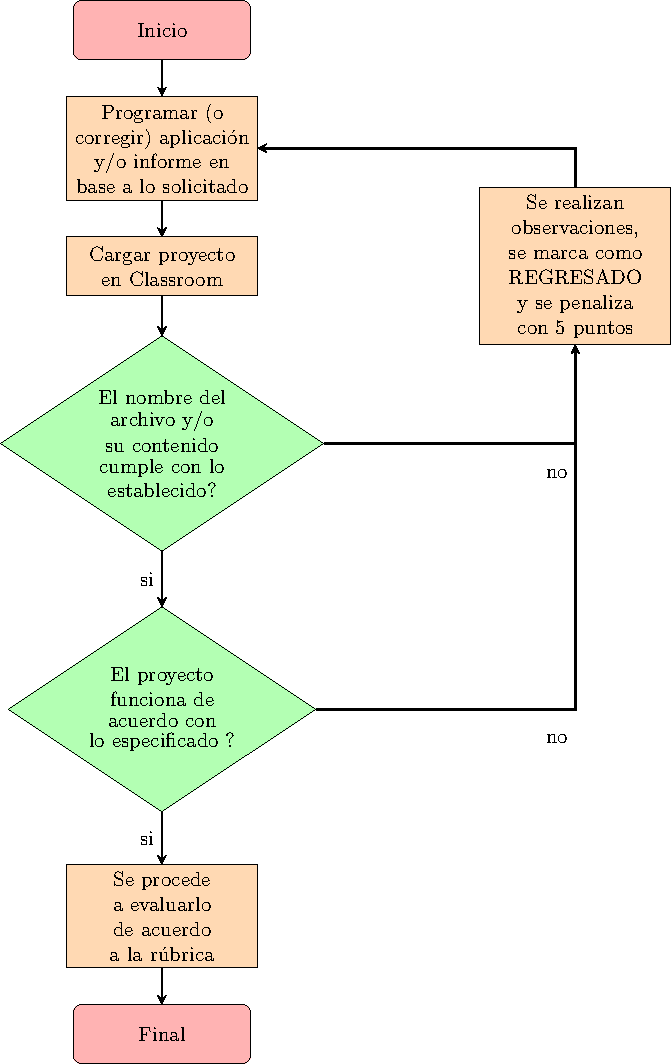
\includegraphics[width=4cm]{DiagramaFlujoVaginal/DF.pdf}
\small
\begin{tabular}{p{5cm}|p{3cm}}
\hline
\textbf{Detalle} & \textbf{Puntos de penalización sobre calificación final} \\
\hline
Nombre Archivo & 8 \\ \hline
Tipo de Archivo & 7 \\ \hline
Estructura de Directorios  & 6 \\ \hline
Falta o Error en Script  & 6 \\ \hline
Poner ZIPs dentro del ZIP  & 8 \\ \hline
Incluir ejecutables (aplica solo cuando el lenguaje es C++)  & 8 \\
\hline
\hline
\end{tabular}
\end{column}
\end{columns}
\end{frame}




\begin{frame}
\frametitle{Premio a la Compresión Lectora 2024}
A pesar de las instrucciones en esta presentación, alguien va a hacer las cosas mal
\begin{center}
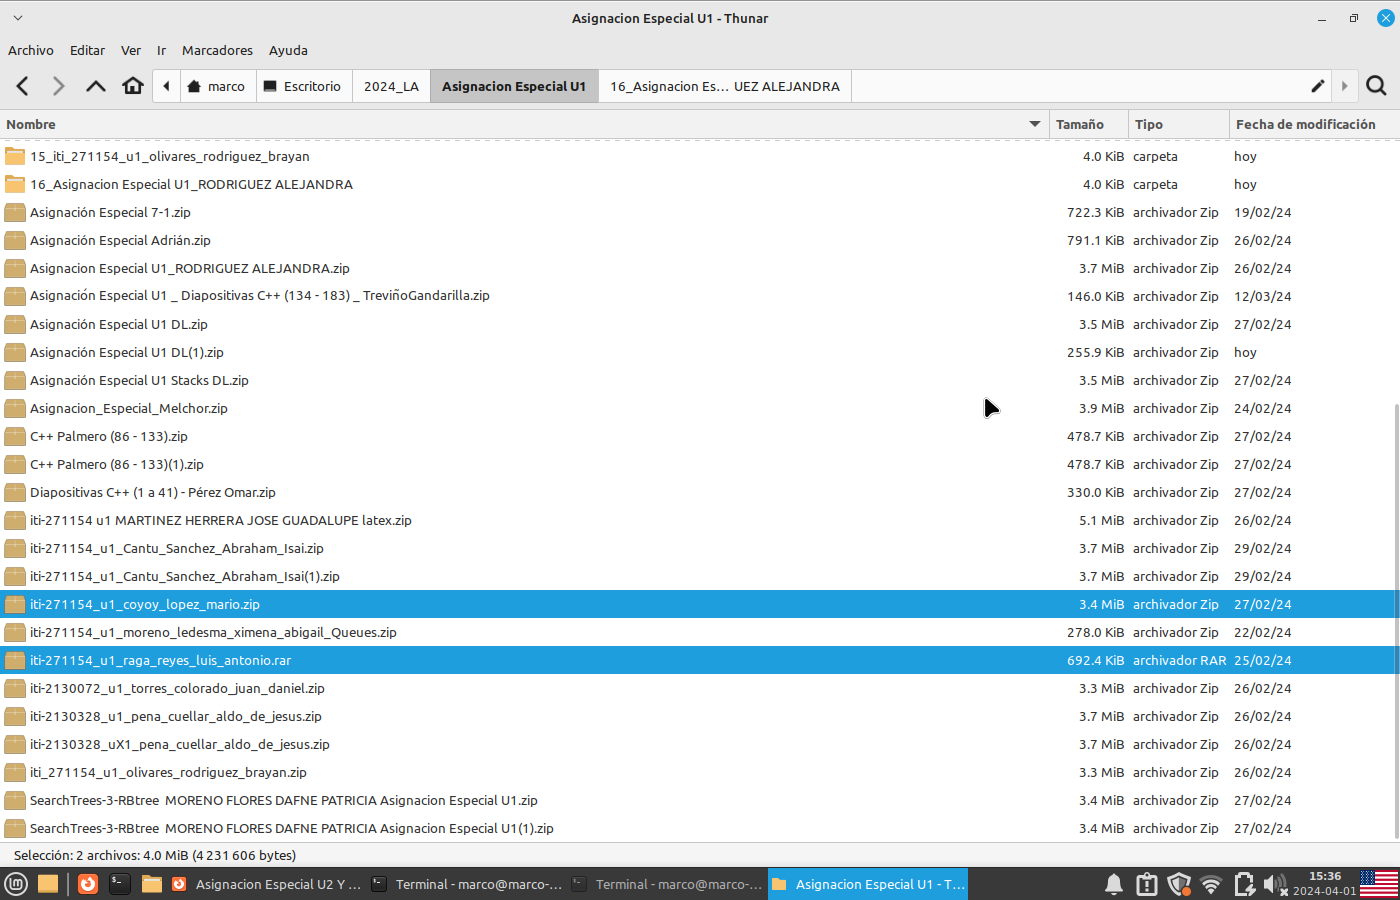
\includegraphics[width=0.75\linewidth]{Entregables/PremioAlaComprensionLectora_2024.png}
\end{center}


\end{frame}


\begin{frame}
\frametitle{Salon de la Fama de Entregas Completas e Incompletas}
\begin{columns}
\begin{column}{0.5\textwidth}
\begin{center}
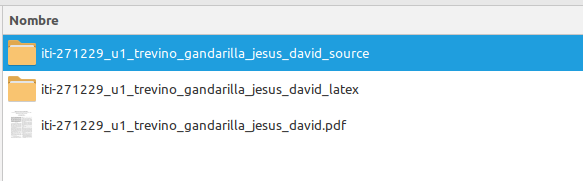
\includegraphics[width=5cm]{Entregables/CasoBien5.png}

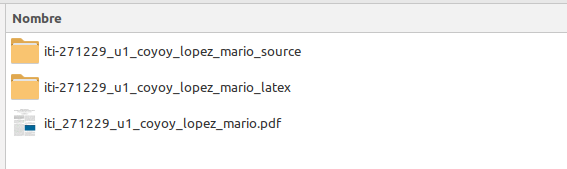
\includegraphics[width=5cm]{Entregables/CasoBien4.png}

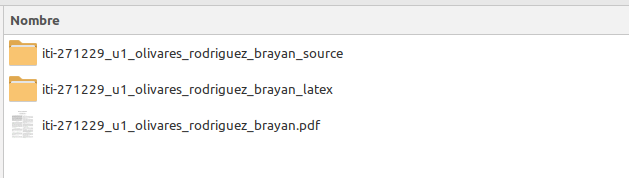
\includegraphics[width=5cm]{Entregables/CasoBien3.png}
\end{center}

\end{column}
\begin{column}{0.5\textwidth}
\begin{center}
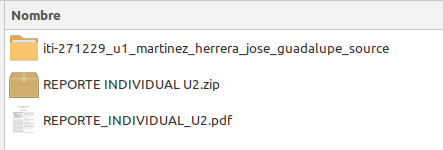
\includegraphics[width=5cm]{Entregables/CasoMal1.png}

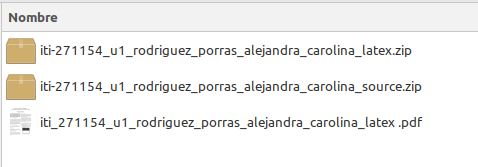
\includegraphics[width=5cm]{Entregables/CasoMal2.png}

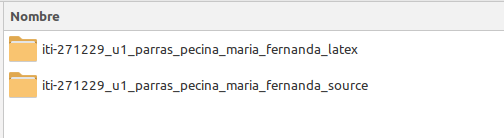
\includegraphics[width=5cm]{Entregables/CasoMal3.png}
\end{center}

\end{column}
\end{columns}
\end{frame}







